%%%%%%%%%%%%%%%%%%%%%%%%%%%%%%%%%%%%%%%%%%%%%%%%%%%
%% P3: Phenomenology of Particle Physics                         
%%
%% Author:  André Rubbia                   		 
%%
%% Figure 5.6 The momentum sphere in the center-of-mass and laboratory frame.
%%
%% This work is licensed under the Creative Commons Attribution 4.0 International License. 
%% To view a copy of this license, visit http://creativecommons.org/licenses/by/4.0/ or 
%% send a letter to Creative Commons, PO Box 1866, Mountain View, CA 94042, USA.
%%
%%%%%%%%%%%%%%%%%%%%%%%%%%%%%%%%%%%%%%%%%%%%%%%%%%%

\documentclass[a4paper,10pt]{article}

\usepackage[T1]{fontenc}
\usepackage[utf8]{inputenc}
\usepackage{lmodern}
\usepackage[labelfont=bf]{caption}
\usepackage{upgreek}

\usepackage{tikz}
\usepackage{pgfplots}
\pgfplotsset{compat=1.17}
\usepgfplotslibrary{ternary}
\usepgfplotslibrary{fillbetween}
\usepgfplotslibrary{external}
\usetikzlibrary{patterns}
\usetikzlibrary{decorations.pathmorphing}
\usetikzlibrary{decorations.markings}
\usetikzlibrary{arrows}
\usetikzlibrary{svg.path}
\usetikzlibrary{shapes}
\usetikzlibrary{arrows.meta}
% define the arrow style
\tikzset{
    arrow/.style={
        decoration={
            markings,
            mark=at position .5 with {
                \arrow[#1, scale=1.5]{latex}
            }
        },
        postaction={decorate},
    }
}
\tikzset{
    arrow flipped/.style={
        decoration={
            markings,
            mark=at position .5 with {
                \arrow[#1, scale=1.5]{latex reversed}
            }
        },
        postaction={decorate},
    }
}
\pgfkeys{/pgf/number format/.cd,1000 sep={}}\usepackage{pgfplots}

\def\d{\mathrm{d}}

\begin{document}

%%%%%%%%%%%%%%%%   FIGURE  %%%%%%%%%%%%%%%%%%%%%%%%%%%%%%
\begin{figure}[htbp]
\begin{center}
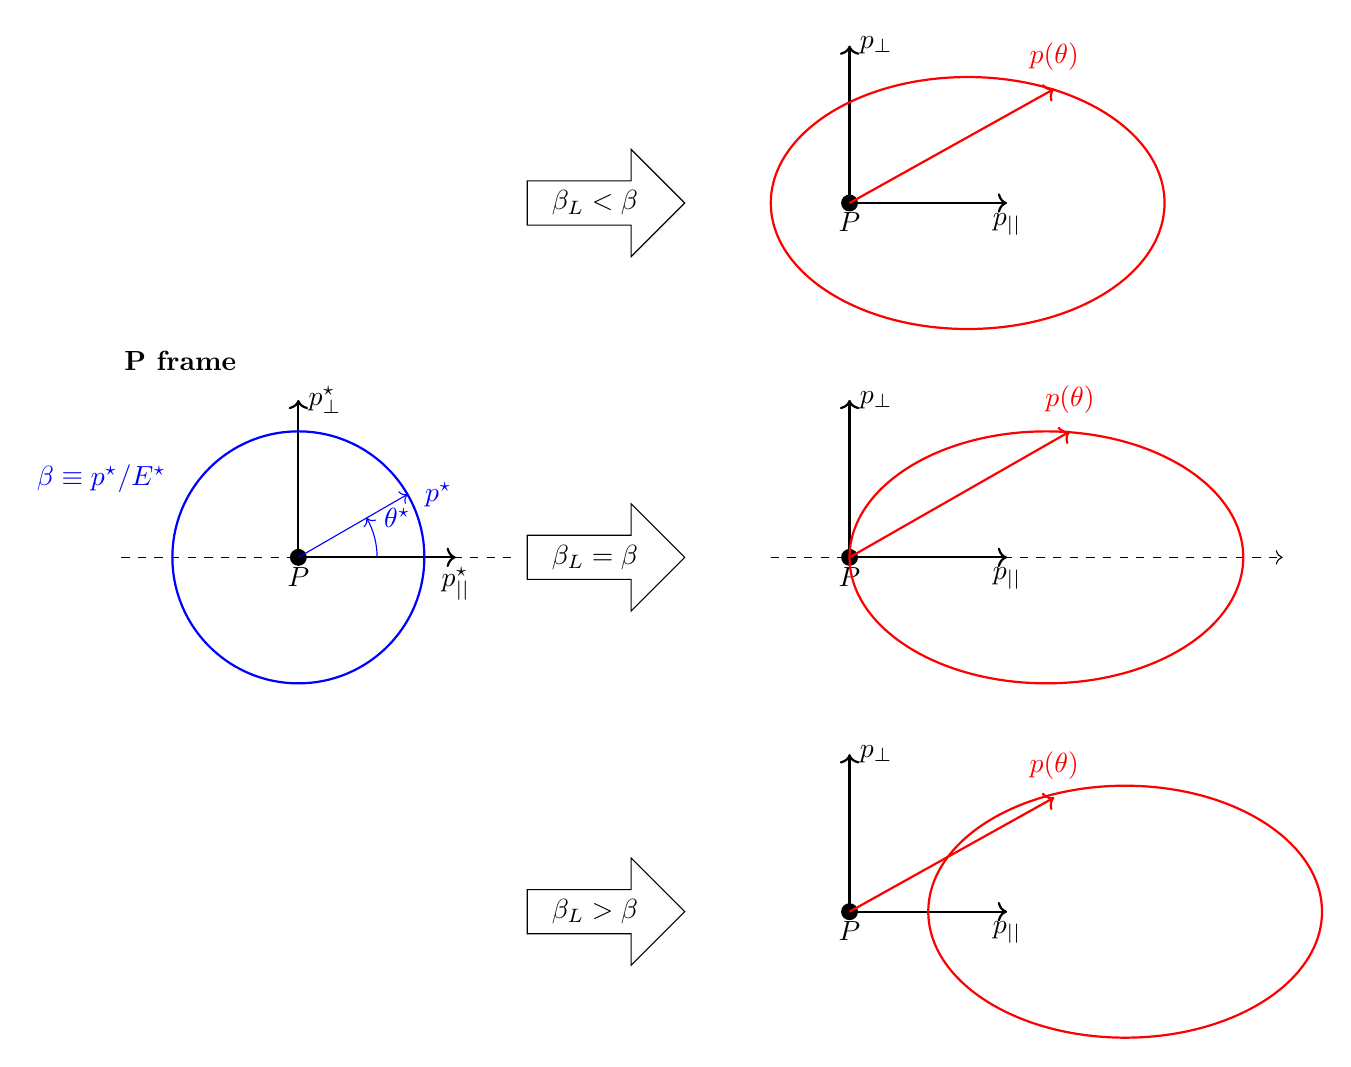
\begin{tikzpicture}[scale=1]
\draw[dashed] (-2.25,0) -- (2.8,0);

\node (X) at (2,1.5) {};

\filldraw (0,0) circle (1mm) node [below] {$P$};
\node at (-1.5,2.5) {\textbf{P frame}};
\draw[black,->,thick] (0,0) -- +(0:2) node [below] {$p^{\star}_{||}$};
\draw[black,->,thick] (0,0) -- +(90:2) node [right] {$p^{\star}_{\perp}$};
\draw[dashed,->] (6,0) -- (12.5,0);
\draw[thick,blue] (0,0) circle (1.6);
\draw[blue,->] (1,0) arc(0:30:1) node [right=0.1cm] {$\theta^\star$};
\draw[blue,->] (0,0) -- +(30:1.6) node [right=0.1cm] {$p^\star$};
\node[blue] at (-2.5,1) {$\beta\equiv p^{\star}/E^{\star}$};

\node[draw, single arrow,
              minimum height=20mm, minimum width=8mm,
              single arrow head extend=4mm,
              anchor=west, rotate=0] at (2.9,0) {$\beta_L = \beta$};

\node[draw, single arrow,
              minimum height=20mm, minimum width=8mm,
              single arrow head extend=4mm,
              anchor=west, rotate=0] at (2.9,4.5) {$\beta_L < \beta$};

\node[draw, single arrow,
              minimum height=20mm, minimum width=8mm,
              single arrow head extend=4mm,
              anchor=west, rotate=0] at (2.9,-4.5) {$\beta_L > \beta$};

\begin{scope}[shift={(7,0)}]
\draw[black,->,thick] (0,0) -- +(0:2) node [below] {$p_{||}$};
\draw[black,->,thick] (0,0) -- +(90:2) node [right] {$p_{\perp}$};
\filldraw (0,0) circle (1mm) node [below] {$P$};
\draw[thick,red] (2.5,0) ellipse (2.5 and 1.6);
\draw[thick,red,->] (0,0) -- (2.8,1.6) node [above=0.1cm] {$p(\theta)$};
\end{scope}

\begin{scope}[shift={(7,4.5)}]
\draw[black,->,thick] (0,0) -- +(0:2) node [below] {$p_{||}$};
\draw[black,->,thick] (0,0) -- +(90:2) node [right] {$p_{\perp}$};
\filldraw (0,0) circle (1mm) node [below] {$P$};
\draw[thick,red] (1.5,0) ellipse (2.5 and 1.6);
\draw[thick,red,->] (0,0) -- (2.6,1.45) node [above=0.1cm] {$p(\theta)$};
\end{scope}

\begin{scope}[shift={(7,-4.5)}]
\draw[black,->,thick] (0,0) -- +(0:2) node [below] {$p_{||}$};
\draw[black,->,thick] (0,0) -- +(90:2) node [right] {$p_{\perp}$};
\filldraw (0,0) circle (1mm) node [below] {$P$};
\draw[thick,red] (3.5,0) ellipse (2.5 and 1.6);
\draw[thick,red,->] (0,0) -- (2.6,1.45) node [above=0.1cm] {$p(\theta)$};
\end{scope}

\end{tikzpicture}
\caption{The momentum sphere in the center-of-mass and laboratory frame for the three
cases $\beta < \beta_L$, $\beta = \beta_L$, and $\beta > \beta_L$.}
\end{center}
\end{figure}
%%%%%%%%%%%%%%%%   END FIGURE  %%%%%%%%%%%%%%%%%%%%%%%%%%%%%%

\end{document}
